% Based on the answer by qubyte at 
% http://tex.stackexchange.com/questions/9767/whats-a-good-package-for-typesetting-quantum-circuits
\documentclass[12pt]{standalone}
\usepackage{tikz}

\usetikzlibrary{backgrounds}
% Dirac Kets
\newcommand{\ket}[1]{\ensuremath{\left|#1\right\rangle}}

\begin{document}
    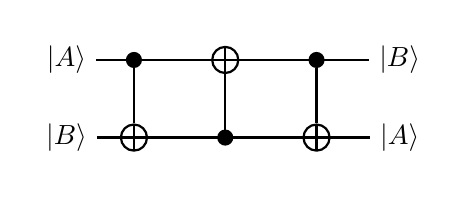
\begin{tikzpicture}[thick,cross/.style={path picture={ 
  \draw[black]
(path picture bounding box.south) -- (path picture bounding box.north);
}}]

    % `operator' will only be used by most gates.
    % `cnot' will refer to CNOT gates.
    % `phase' is used for controlled gates.
    \tikzstyle{operator} = [draw,fill=white,minimum size=1.5em]
    \tikzstyle{cnot} = [draw,cross,circle,minimum size=5pt]
      \tikzstyle{phase} = [draw,fill,shape=circle,minimum size=5pt,inner sep=0pt]
    %
    \matrix[row sep=0.4cm, column sep=0.8cm] (circuit) {

    % First row.
    \node (q1) {\ket{A}}; &[-0.5cm] 
    \node[phase] (P11) {}; &
    \node[cnot] (C12) {}; &
    \node[phase] (P13) {}; &[-0.3cm] 
    \node (q1end) {\ket{B}};\\

    % Second row.
    \node (q2) {\ket{B}}; &
    \node[cnot] (C21) {}; &
    \node[phase] (P22) {}; &
    \node[cnot] (C23) {}; &[-0.3cm] 
    \node (q2end) {\ket{A}}; \\
    };

    \begin{pgfonlayer}{background}
        % Draw lines.
        \draw[thick] (q1) -- (q1end)  (q2) -- (q2end) (P11) -- (C21) (C12) -- (P22) (P13) -- (C23);
    \end{pgfonlayer}
    %
    \end{tikzpicture}
\end{document}
